\section{Afgrænsning}\label{sec:afgraensning}

% Magnus
\subsection{Grundlæggende del: \textsc{SimpDam}}
I den grundlæggende del konstruerede vi et simpelt damspil, hvor interaktionen med brugerne foregår via en grafisk brugergrænseflade implementeret med \texttt{JavaFX}. Brætstørrelsen $n \in \{3, .. , 100\}$ sættes af brugeren. Vi har vedhæftet to udgaver af \textsc{SimpDam}: En \texttt{.jar}-fil, hvor $n$ angives som en kommandolinjeparameter, når \texttt{.jar}-filen køres gennem terminalen. Samt en \texttt{Eclipse} projektfil med dertilhørende \texttt{.java}-filer, hvor $n$ efterspørges gennem konsollen i \texttt{Eclipse}.

% Magnus
\subsection{Avanceret del: \textsc{AvaDam}}

Det avancerede damspil har samme grundstruktur som det simple damspil, men vi har udvidet med en del ekstra features. De mest væsentlige features findes på figurerne \ref{fig:features1} og \ref{fig:features2}, og uddybes i afsnittene Design og Implementering. \\
\begin{figure}[H]
\centering
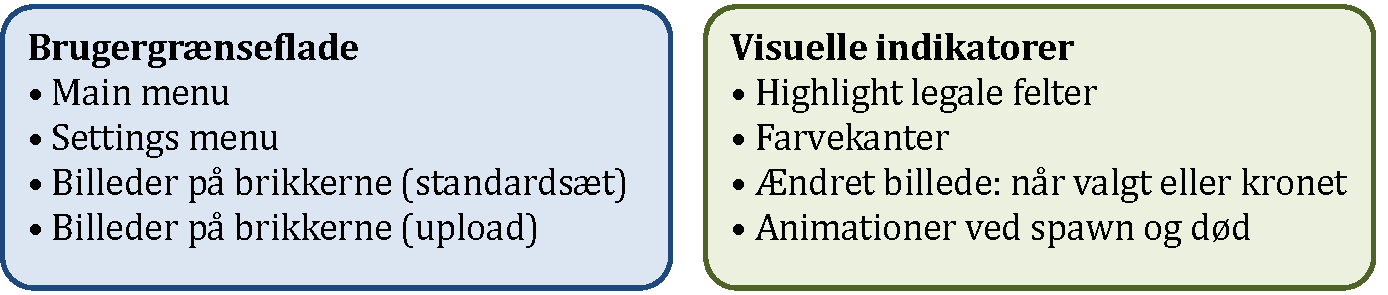
\includegraphics[width = 1.0  \textwidth]{Figurer/features1.pdf}
\caption{Yderligere implementeringer efter \textsc{SimpDam}. Del 1 af 2.}
\label{fig:features1}
\end{figure}

\begin{figure}[H]
\centering
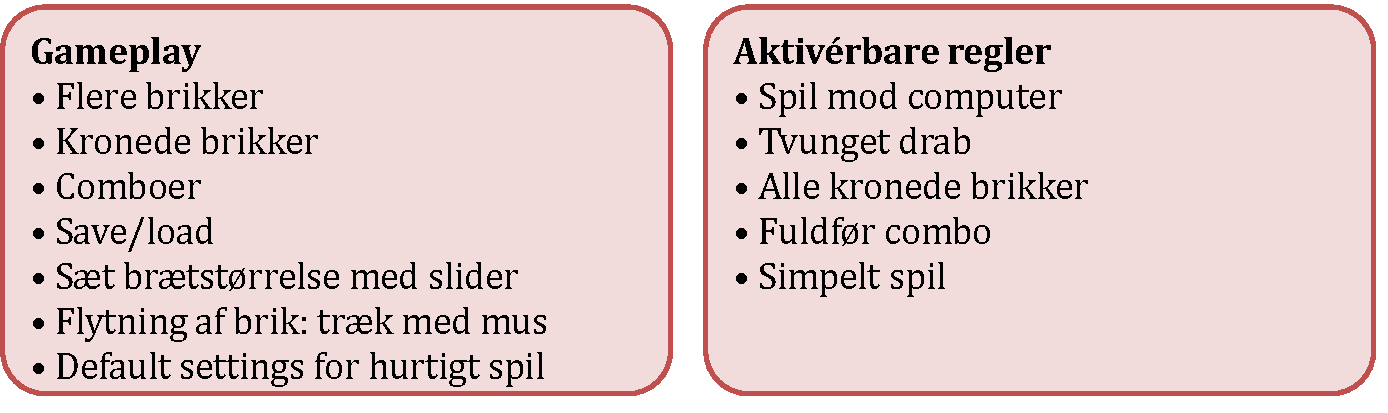
\includegraphics[width = 1.0  \textwidth]{Figurer/features2.pdf}
\caption{Yderligere implementeringer efter \textsc{SimpDam}. Del 2 af 2.}
\label{fig:features2}
\end{figure}
